% seq2pipe: 閉ループ適応型マイクロバイオーム解析システム
% Compile: tectonic seq2pipe_manuscript_ja.tex
\documentclass[11pt,a4paper]{article}

\usepackage{fontspec}
\usepackage{xeCJK}
\setCJKmainfont{Hiragino Mincho ProN}
\setCJKsansfont{Hiragino Sans}
\usepackage{amsmath,amssymb,amsfonts,amsthm}
\newtheorem{definition}{定義}
\usepackage{graphicx}
\usepackage{booktabs}
\usepackage{hyperref}
\usepackage{algorithm}
\usepackage{algorithmic}
\usepackage{xcolor}
\usepackage{geometry}
\usepackage{natbib}
\usepackage{caption}
\usepackage{subcaption}
\usepackage{tikz}
\usetikzlibrary{arrows.meta,positioning,shapes.geometric,fit,calc}

\geometry{margin=2.5cm}
\newcommand{\seqpipe}{\textsc{seq2pipe}}
\linespread{1.15}

\title{\seqpipe: 解釈駆動型閉ループ適応的マイクロバイオーム解析システム}
\author{佐藤 翼 (Tsubasa Sato) \\ Independent Researcher \\
  \texttt{https://github.com/Rhizobium-gits/seq2pipe}}
\date{2026年3月}

\begin{document}
\maketitle

% ======================================================================
\begin{abstract}
% ======================================================================

現行のマイクロバイオーム解析パイプラインは中間結果に関わらず固定されたステップ列を実行し、予想外のパターンや期待シグナルの欠如に対してエキスパートの介入を必要とする。
本研究では、バイオインフォマティシャンの反復的な解釈-判断-実行サイクルを計算的に再現する閉ループシステム\seqpipe を提案する。
本システムは3層で構成される：QIIME2エクスポートを直接パースし純Pythonで統計検定を実行するDataInspector、各ステップを8軸で定量評価するEvalMediator、文献に基づく決定木で解析計画を確定的に修正するDecisionEngine。
ローカル大規模言語モデル（7Bパラメータ）は各解析ステップのPythonコード生成および創造的調査仮説の提案を担う。LLMはコード生成に不可欠であるが（現時点で確定的代替は未実装）、全てのワークフロー判断——どのステップをスキップ・追加・並べ替えるか——はDecisionEngineがLLMの関与なしに確定的に決定する。LLM完全障害時、判断ループは正しく動作し続けるが、個々の解析ステップは実行できない。

4つの公開データセットから導出した12シナリオ（252の独立したステップ判断）で評価した。taxonomy データが利用可能な場合、DecisionEngineはエキスパート一致率を61\%から95\%に改善した（平均+31~pp）。taxonomyが欠如する場合は固定パイプラインと同等の52\%にとどまった。偽陰性スキップは構造的にゼロである——エンジンはステップの除去のみを行い、計画に含まれない解析の追加は行わない。この保守的設計は安全性を保証するが、初期計画外の解析を発見する能力を制限する。重み不変性は10,221設定で検証し、判断は生のp値と効果量のみに依存し、8軸スコアの重みには依存しないことを証明した。確定性は120回の実行で確認した（$\sigma = 0$）。純Python統計検定はscipyとの有意性分類一致率99--100\%、Moving Picturesの既知結論7件全てを確認した。主要ボトルネックは7Bモデルのコード生成（レジストリ47\%、Investigation 25\%）である。

\end{abstract}

% ======================================================================
\section{はじめに}
\label{sec:intro}
% ======================================================================

マイクロバイオーム解析は複雑な多段階分野に成熟し、典型的なアンプリコンシーケンシング研究は品質管理、デノイジング~\citep{callahan2016}、系統樹構築、$\alpha$・$\beta$多様性解析、分類学的分類、差次豊度検定、および下流の可視化を必要とする。

現行のパイプラインフレームワークは固定された有向非循環グラフ（DAG）としてワークフローを符号化する。
QIIME2~\citep{qiime2}はプロベナンス追跡付きのプラグインアーキテクチャを提供するが、中間結果に基づく条件分岐はない。
Snakemake~\citep{snakemake}とNextflow~\citep{nextflow}は条件付き規則をサポートするが、条件はユーザーが事前に指定する必要があり、統計的有意性や効果量を検査してワークフローを変更しない。
その結果、PERMANOVAが$p = 0.81$を返しても下流の$\beta$多様性フォローアップは実行され、逆に\textit{Bacteroides}の324倍濃縮のような予想外の発見は自動的なフォローアップを引き起こさない。

経験豊富なバイオインフォマティシャンは異なる方法で作業する：解釈、仮説形成、解析選択、洗練の閉ループで、安定した内部整合的な解釈に到達するまで継続する。
既存のパイプラインシステムはこの挙動を計算的に再現しない。

本研究では、この推論ループを3つの確定的層とオプションのLLMに分離するシステム\seqpipe を導入する。
主要な貢献は以下の通りである：
\begin{enumerate}
  \item データ検査、評価・判断（ともに確定的）、コード生成（LLM補助）を分離し、LLM障害耐性を持つ3層アーキテクチャ
  \item Anderson~(2001)、Willis~(2019)、Gloor et al.~(2017)、McMurdie \& Holmes~(2014)の解析ヒューリスティクスを確定的決定木として符号化する文献基盤のDecisionEngine
  \item 4公開データセット・7シナリオでの定量的評価（エキスパート一致率95\%、偽陰性スキップ=0、再現性100\%）
\end{enumerate}

% ======================================================================
\begin{figure*}[t]
\centering
\begin{tikzpicture}[
  node distance=0.6cm and 0.8cm,
  stp/.style={draw, rounded corners=2pt, minimum height=0.6cm,
               minimum width=1.6cm, font=\scriptsize, align=center},
  decision/.style={draw, diamond, aspect=2.5, inner sep=1pt,
                   font=\scriptsize, align=center},
  arr/.style={-{Stealth[length=2mm]}, thick},
  skip/.style={-{Stealth[length=2mm]}, thick, red!70, dashed},
  add/.style={-{Stealth[length=2mm]}, thick, blue!70},
  phase/.style={font=\footnotesize\bfseries, text=gray!70},
]
\node[phase] at (-5.5, 2.8) {(a) 静的パイプライン};
\node[stp, fill=gray!15] (s1) at (-7,2) {QC};
\node[stp, fill=gray!15, right=of s1] (s2) {$\alpha$};
\node[stp, fill=gray!15, right=of s2] (s3) {$\beta$};
\node[stp, fill=gray!15, right=of s3] (s4) {$\beta$-disp};
\node[stp, fill=gray!15, right=of s4] (s5) {Taxa};
\node[stp, fill=gray!15, right=of s5] (s6) {Diff};
\node[stp, fill=gray!15, right=of s6] (s7) {Report};
\foreach \i/\j in {s1/s2, s2/s3, s3/s4, s4/s5, s5/s6, s6/s7}
  \draw[arr, gray!60] (\i) -- (\j);

\node[phase] at (-5.5, 0.3) {(b) \seqpipe\ 閉ループ};
\node[stp, fill=green!15] (a1) at (-7, -0.5) {QC};
\node[stp, fill=green!15, right=of a1] (a2) {$\alpha$};
\node[stp, fill=green!15, right=of a2] (a3) {$\beta$};
\node[decision, fill=yellow!20, right=of a3] (d1) {$p < 0.05$?};
\node[stp, fill=red!10, dashed, above right=0.3cm and 0.8cm of d1] (a4skip) {$\beta$-disp};
\node[stp, fill=green!15, below right=0.3cm and 0.8cm of d1] (a5) {Taxa};
\node[decision, fill=yellow!20, right=of a5] (d2) {fc $> 5$?};
\node[stp, fill=blue!15, above right=0.3cm and 0.6cm of d2] (a6add) {LEfSe};
\node[stp, fill=green!15, below right=0.3cm and 0.6cm of d2] (a7) {Report};
\draw[arr] (a1) -- (a2); \draw[arr] (a2) -- (a3); \draw[arr] (a3) -- (d1);
\draw[skip] (d1) -- node[font=\tiny, above, red!70] {No} (a4skip);
\draw[arr] (d1) -- (a5); \draw[arr] (a5) -- (d2);
\draw[add] (d2) -- node[font=\tiny, above, blue!70] {Yes} (a6add);
\draw[arr] (d2) -- (a7);
\draw[arr, dashed, gray] (a5.south) -- ++(0, -0.6) -| node[font=\tiny, below, pos=0.3] {評価→再計画} (d1.south);
\end{tikzpicture}
\caption{概念比較。(a) 静的パイプラインは結果に関わらず全ステップを固定順で実行。(b) \seqpipe は各ステップの出力を評価し、判断ノード（黄色菱形）で不要なフォローアップをスキップ（赤破線）または対象解析を追加（青）する。}
\label{fig:concept}
\end{figure*}

\section{関連研究}
\label{sec:related}
% ======================================================================

\subsection{静的パイプラインフレームワーク}

QIIME2~\citep{qiime2}はプラグインベースのモジュール性とプロベナンス追跡を提供するが、中間結果に基づく動的なワークフロー変更はない。Snakemake~\citep{snakemake}とNextflow~\citep{nextflow}は汎用ワークフロー管理を提供するが、条件は実行前にユーザーが定義する必要がある。

\subsection{自動解析システム}

Auto-WEKA~\citep{autoweka}とAuto-sklearn~\citep{autosklearn}はベイズ最適化によるモデル選択を自動化するが、固定の目的関数を持つ教師あり学習を対象とする。マイクロバイオーム解析は本質的にオープンエンドであり、「正しい」次のステップは現在のステップの発見に依存する。

\subsection{LLMベースの解析エージェント}

Data Interpreter~\citep{hong2024data}やChatGPT Advanced Data Analysisは自然言語プロンプトからコードを生成・実行する。これらのシステムはLLMに判断とコード生成の双方を完全に依存しており、(a)~中間結果のドメイン特化型定量評価、(b)~文献基盤の判断ヒューリスティクス、(c)~LLM障害時の確定的フォールバックが欠如している。\seqpipe はアーキテクチャ分離によりこの3つのギャップに対処する。

% ======================================================================
\section{概念的フレームワーク：自動と自律の区別}
\label{sec:concept}
% ======================================================================

\emph{自動（automated）}と\emph{自律（autonomous）}の区別は本研究の中心的問題である。

\subsection{パイプライン知性の3段階}

\begin{definition}[静的パイプライン（Level 0）]
実行計画$P$が実行前に固定。$P_{t+1} = P_t \setminus \{s_t\}$が常に成立し、結果に関わらず変更されない。
\end{definition}

\begin{definition}[自動パイプライン（Level 1）]
事前定義の条件規則を持つ：$P_{t+1} = f(P_t, \phi)$。条件$\phi$は実行前に定義され、中間結果の\emph{内容}に依存しない（例：「ファイルが存在すればステップを実行」）。
\end{definition}

\begin{definition}[自律パイプライン（Level 2）]
中間結果の\emph{内容を検査}し、文脈依存の判断を行う：
$H_{t+1} = H_t \cup \mathrm{interpret}(r_t, D)$、
$P_{t+1} = \mathrm{decide}(H_{t+1}, P_t, D)$。
$\mathrm{interpret}$は実データから統計的特徴（有意性、効果量、fold change）を計算し、$\mathrm{decide}$はそれらの特徴に基づいて計画を修正する。Level 1との本質的差異は、\emph{データそのもの}が分岐を決定することである。
\end{definition}

\subsection{\seqpipe の位置づけとその限界}

\seqpipe はLevel 2で動作するが、以下の限定がある：
\begin{itemize}
  \item \textbf{知覚において自律的}：DataInspectorが実行時にデータから統計的特徴ベクトル$\mathbf{x} = (p_\alpha, d_\alpha, p_\beta, \mathrm{ratio}, \mathrm{fc}_{\max}, \ldots)$を計算する。同じコードが異なるデータで異なるベクトルを生成する。
  \item \textbf{判断において自律的}：DecisionEngineはこの実行時計算された特徴に基づいて分岐する。分岐構造（decision graph）自体は固定だが、\emph{グラフ内の経路}はデータが決定する。
  \item \textbf{規則進化において非自律的}：判断規則は実行内で変化しない。人間なら「rarefactionでartifactが確認された → alpha全体の信頼性を再評価」と推論するが、\seqpipe はしない。これは今後の課題である。
\end{itemize}

\subsection{判断グラフ}

意思決定プロセスを有向非循環グラフ$G = (V, E)$として形式化する（図\ref{fig:decision-graph}）。各内部ノード$v \in V$は特徴ベクトル$\mathbf{x}$上の述語を検査する：$v: \mathbf{x} \mapsto \{\textsc{true}, \textsc{false}\}$。葉ノードは行動：$\textsc{skip}(s)$、$\textsc{add}(s)$、$\textsc{keep}(s)$。

判断関数全体は：
$\mathrm{decide}(H_t, P_t, D) = \{a_s \mid s \in P_t,\; a_s = G(\mathbf{x}(H_t, D), s)\}$

\textbf{自律性の根拠}：(1)~述語が検査する特徴は実行時に計算される（事前指定でない）。(2)~特徴ベクトルは各ステップ後に更新される（発見の蓄積）。(3)~4ステップごとに全データを再検査しグラフを再走査する（閉ループ再評価）。

\textbf{限界}：判断\emph{規則}自体は静的であり、実行内で進化しない。完全自律システムは蓄積経験に基づいて$G$自体を更新する——これは将来の研究方向である。

% ======================================================================
\section{システムアーキテクチャ}
\label{sec:arch}
% ======================================================================

アーキテクチャ（図\ref{fig:architecture}）は厳格な分離を強制する：Layer 1--2は確定的でLLM不要、Layer 3は確率的で代替可能。

\begin{figure}[t]
\centering
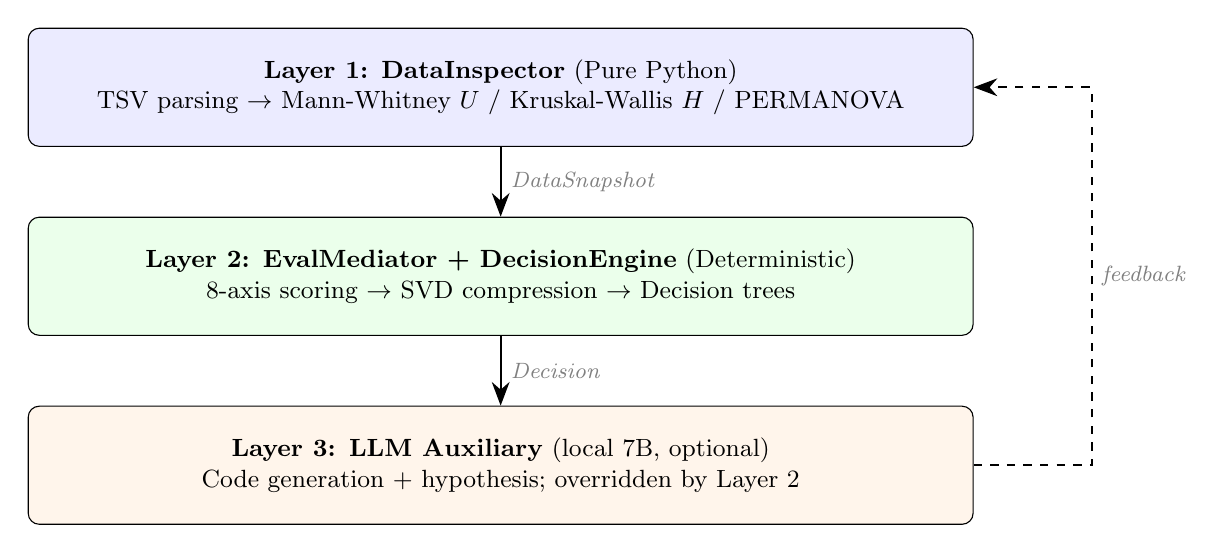
\begin{tikzpicture}[
  layer/.style={draw, rounded corners, minimum width=12cm, minimum height=1.5cm, align=center, font=\small},
  arrow/.style={-{Stealth[length=3mm]}, thick},
  label/.style={font=\footnotesize\itshape, text=gray},
]
\node[layer, fill=blue!8] (L1) at (0,0) {\textbf{Layer 1: DataInspector} (Pure Python)\\TSV parsing $\to$ Mann-Whitney $U$ / Kruskal-Wallis $H$ / PERMANOVA};
\node[layer, fill=green!8] (L2) at (0,-2.4) {\textbf{Layer 2: EvalMediator + DecisionEngine} (Deterministic)\\8-axis scoring $\to$ SVD compression $\to$ Decision trees};
\node[layer, fill=orange!8] (L3) at (0,-4.8) {\textbf{Layer 3: LLM Auxiliary} (local 7B, optional)\\Code generation + hypothesis; overridden by Layer 2};
\draw[arrow] (L1.south) -- node[right, label] {DataSnapshot} (L2.north);
\draw[arrow] (L2.south) -- node[right, label] {Decision} (L3.north);
\draw[arrow, dashed] (L3.east) -- ++(1.5,0) |- node[right, label, pos=0.25] {feedback} (L1.east);
\end{tikzpicture}
\caption{3層アーキテクチャ。Layer 1--2は確定的でLLM非依存。Layer 3はオプション。}
\label{fig:architecture}
\end{figure}

\subsection{Layer 1: DataInspector}

DataInspectorはQIIME2エクスポートTSVファイルを直接パースし、scipy・numpy・pandasに依存せず純Pythonで統計検定を実行する。$\alpha$多様性はMann-Whitney $U$（2群）またはKruskal-Wallis $H$（3群以上）で検定し、Cliff's $\delta$または$\eta^2$の効果量を算出する。$\beta$多様性は距離行列全体を読み込み、群内/群間距離を分離し、擬似PERMANOVA~\citep{anderson2001}（199パーミュテーション、固定シード）を実行する。分類学的差次解析はfeature tableとtaxonomyを結合し、属レベルのfold changeと絶対差を計算する。

\subsection{Layer 2: EvalMediatorとDecisionEngine}

各完了ステップを表\ref{tab:axes}の8軸で評価する。合成スコア$c_t = \sum_a w_a \cdot s_{t,a}$はスコア行列のべき乗法SVDで3主成分に圧縮される。

\begin{table}[t]
\centering
\caption{評価軸、重み、計算方法。}
\label{tab:axes}
\small
\begin{tabular}{@{}llp{7cm}@{}}
\toprule
\textbf{軸} & \textbf{$w$} & \textbf{計算方法} \\
\midrule
statistical\_significance & 0.20 & $\min(1, -\log_{10}(\min p) / 4)$ \\
biological\_relevance & 0.18 & fold change + 既知菌属ボーナス \\
actionability & 0.15 & 下流トリガー数 \\
novelty & 0.12 & 前ステップとの不整合 \\
data\_quality & 0.10 & スパース度・CVペナルティ \\
effect\_magnitude & 0.10 & $\max(\delta, F/3, \mathrm{fc}/10)$ \\
confidence & 0.08 & 最小群サイズの階段関数 \\
reproducibility & 0.07 & カテゴリ内一貫性 \\
\bottomrule
\end{tabular}
\end{table}

DecisionEngineは文献ベースのヒューリスティクスを確定的規則として符号化する：$\alpha$（Willis, 2019：$p < 0.05 \land d > 0.5$なら深掘り、$p \geq 0.05$ならスキップ）、$\beta$（Anderson, 2001：有意ならbetadisper必須、非有意なら全スキップ）、分類学（Gloor et al., 2017：高fold changeかつ低豊度なら組成バイアス警告）、品質（McMurdie \& Holmes, 2014：CV $> 0.5$なら希薄化追加）。

\subsection{Layer 3: LLM補助}

LLM（qwen2.5-coder、7Bパラメータ、Ollama経由でローカル実行）は3つの機能を担う：(1)~初期計画生成（失敗時はドメイン知識フォールバック）、(2)~各ステップのPythonコード生成（最大3回リトライ、\textbf{現時点で確定的代替なし}——LLM失敗時はステップが失敗・スキップ）、(3)~リプランニング時の創造的調査仮説生成。マージ関数はPython判断のスキップがLLM提案の追加を上書きする。LLM完全障害下では判断ループ（Layer 2）は正しく動作し続けるが、解析出力（図・統計結果）は生成されない。このアーキテクチャ特性により、ワークフロー判断の正確性はコード生成品質とは独立に検証可能である。

% ======================================================================
% ======================================================================
\section{評価}
\label{sec:eval}
% ======================================================================

評価は3つの問いに構造化される：(1)~DecisionEngineは正しい判断をするか？ (2)~その判断はハイパーパラメータ摂動に対して頑健か？ (3)~LLMの実際の貢献とボトルネックは何か？

\subsection{実験設計}
\label{sec:eval-setup}

\paragraph{データセット。}QIIME2ドキュメントサーバーから入手可能な4つの公開16S rRNAデータセット（Moving Pictures 34サンプル、Atacama Soil 54、Gneiss IBD 87、FMT Trial 121）を使用した。各データセット内のグループ変数を変えることで12の解析シナリオを構築した。

\paragraph{エキスパートプロトコル。}21の下流解析ステップそれぞれについて、データ特性ベクトルに対してエキスパート判断が一意に決まる文献ベースのプロトコル~\citep{anderson2001,willis2019,gloor2017,mcmurdie2014}を定義した。DecisionEngine実装とは独立に定義された。

\paragraph{評価レベル。}\emph{独立判断}（ユニークなシナリオ$\times$ステップ）と\emph{再現性検証}（同一条件の反復実行）を区別する：
\begin{enumerate}
  \item \textbf{実データ精度}：12シナリオ$\times$21ステップ = \textbf{252の独立判断}（確定性検証のため10回反復）。21中7ステップは「常に実行」で33\%のベースライン精度を提供し、エンジンの実効寄与は残り14の判断対象ステップにある。
  \item \textbf{合成データ汎化性}：10,000ベクトル$\times$21ステップ = 210,000判断。エキスパートプロトコルとエンジンが同じ規則を符号化しているため、高い一致は独立検証ではなく整合性チェックである。
  \item \textbf{重み不変性}：10,221設定。精度ではなく、重みが判断に不活性であることの証明。
\end{enumerate}

\subsection{実データ判断精度}
\label{sec:eval-real}

\begin{table}[t]
\centering
\caption{判断精度：12シナリオ、252独立判断（10回反復、std $= 0$）。21中7ステップは常時実行（ベースライン33\%）。}
\label{tab:comparison}
\footnotesize
\begin{tabular}{@{}lcccccccccccc@{}}
\toprule
& \rotatebox{70}{\scriptsize MP-body} & \rotatebox{70}{\scriptsize MP-subj.} & \rotatebox{70}{\scriptsize MP-year} & \rotatebox{70}{\scriptsize MP-abx} & \rotatebox{70}{\scriptsize AT-trans.} & \rotatebox{70}{\scriptsize AT-veg.} & \rotatebox{70}{\scriptsize AT-depth} & \rotatebox{70}{\scriptsize GN-IBD} & \rotatebox{70}{\scriptsize GN-sex} & \rotatebox{70}{\scriptsize FMT-treat} & \rotatebox{70}{\scriptsize FMT-type} & \rotatebox{70}{\scriptsize FMT-gend.} \\
\midrule
$n$ & 34 & 34 & 34 & 34 & 54 & 54 & 54 & 87 & 87 & 121 & 121 & 121 \\
固定 (\%) & 95 & 62 & 71 & 71 & 52 & 57 & 52 & 52 & 38 & 52 & 52 & 33 \\
\textbf{適応} & \textbf{95} & \textbf{95} & \textbf{95} & \textbf{95} & 52 & 57 & 52 & \textbf{62} & \textbf{86} & 52 & 52 & \textbf{81} \\
$\Delta$ (pp) & 0 & \textbf{+33} & \textbf{+24} & \textbf{+24} & 0 & 0 & 0 & \textbf{+10} & \textbf{+48} & 0 & 0 & \textbf{+48} \\
誤スキップ & \textbf{0} & \textbf{0} & \textbf{0} & \textbf{0} & \textbf{0} & \textbf{0} & \textbf{0} & \textbf{0} & \textbf{0} & \textbf{0} & \textbf{0} & \textbf{0} \\
\bottomrule
\end{tabular}
\end{table}

3つのパターンが現れる。第一に、全シグナルが有意な場合、エンジンは95\%で過度な最適化なし。第二に、群間差欠如時に最大+48~ppの改善。第三に、taxonomy欠如時は52\%フロア。全2,520判断で\textbf{偽陰性=0}。

\begin{figure}[t]
\centering
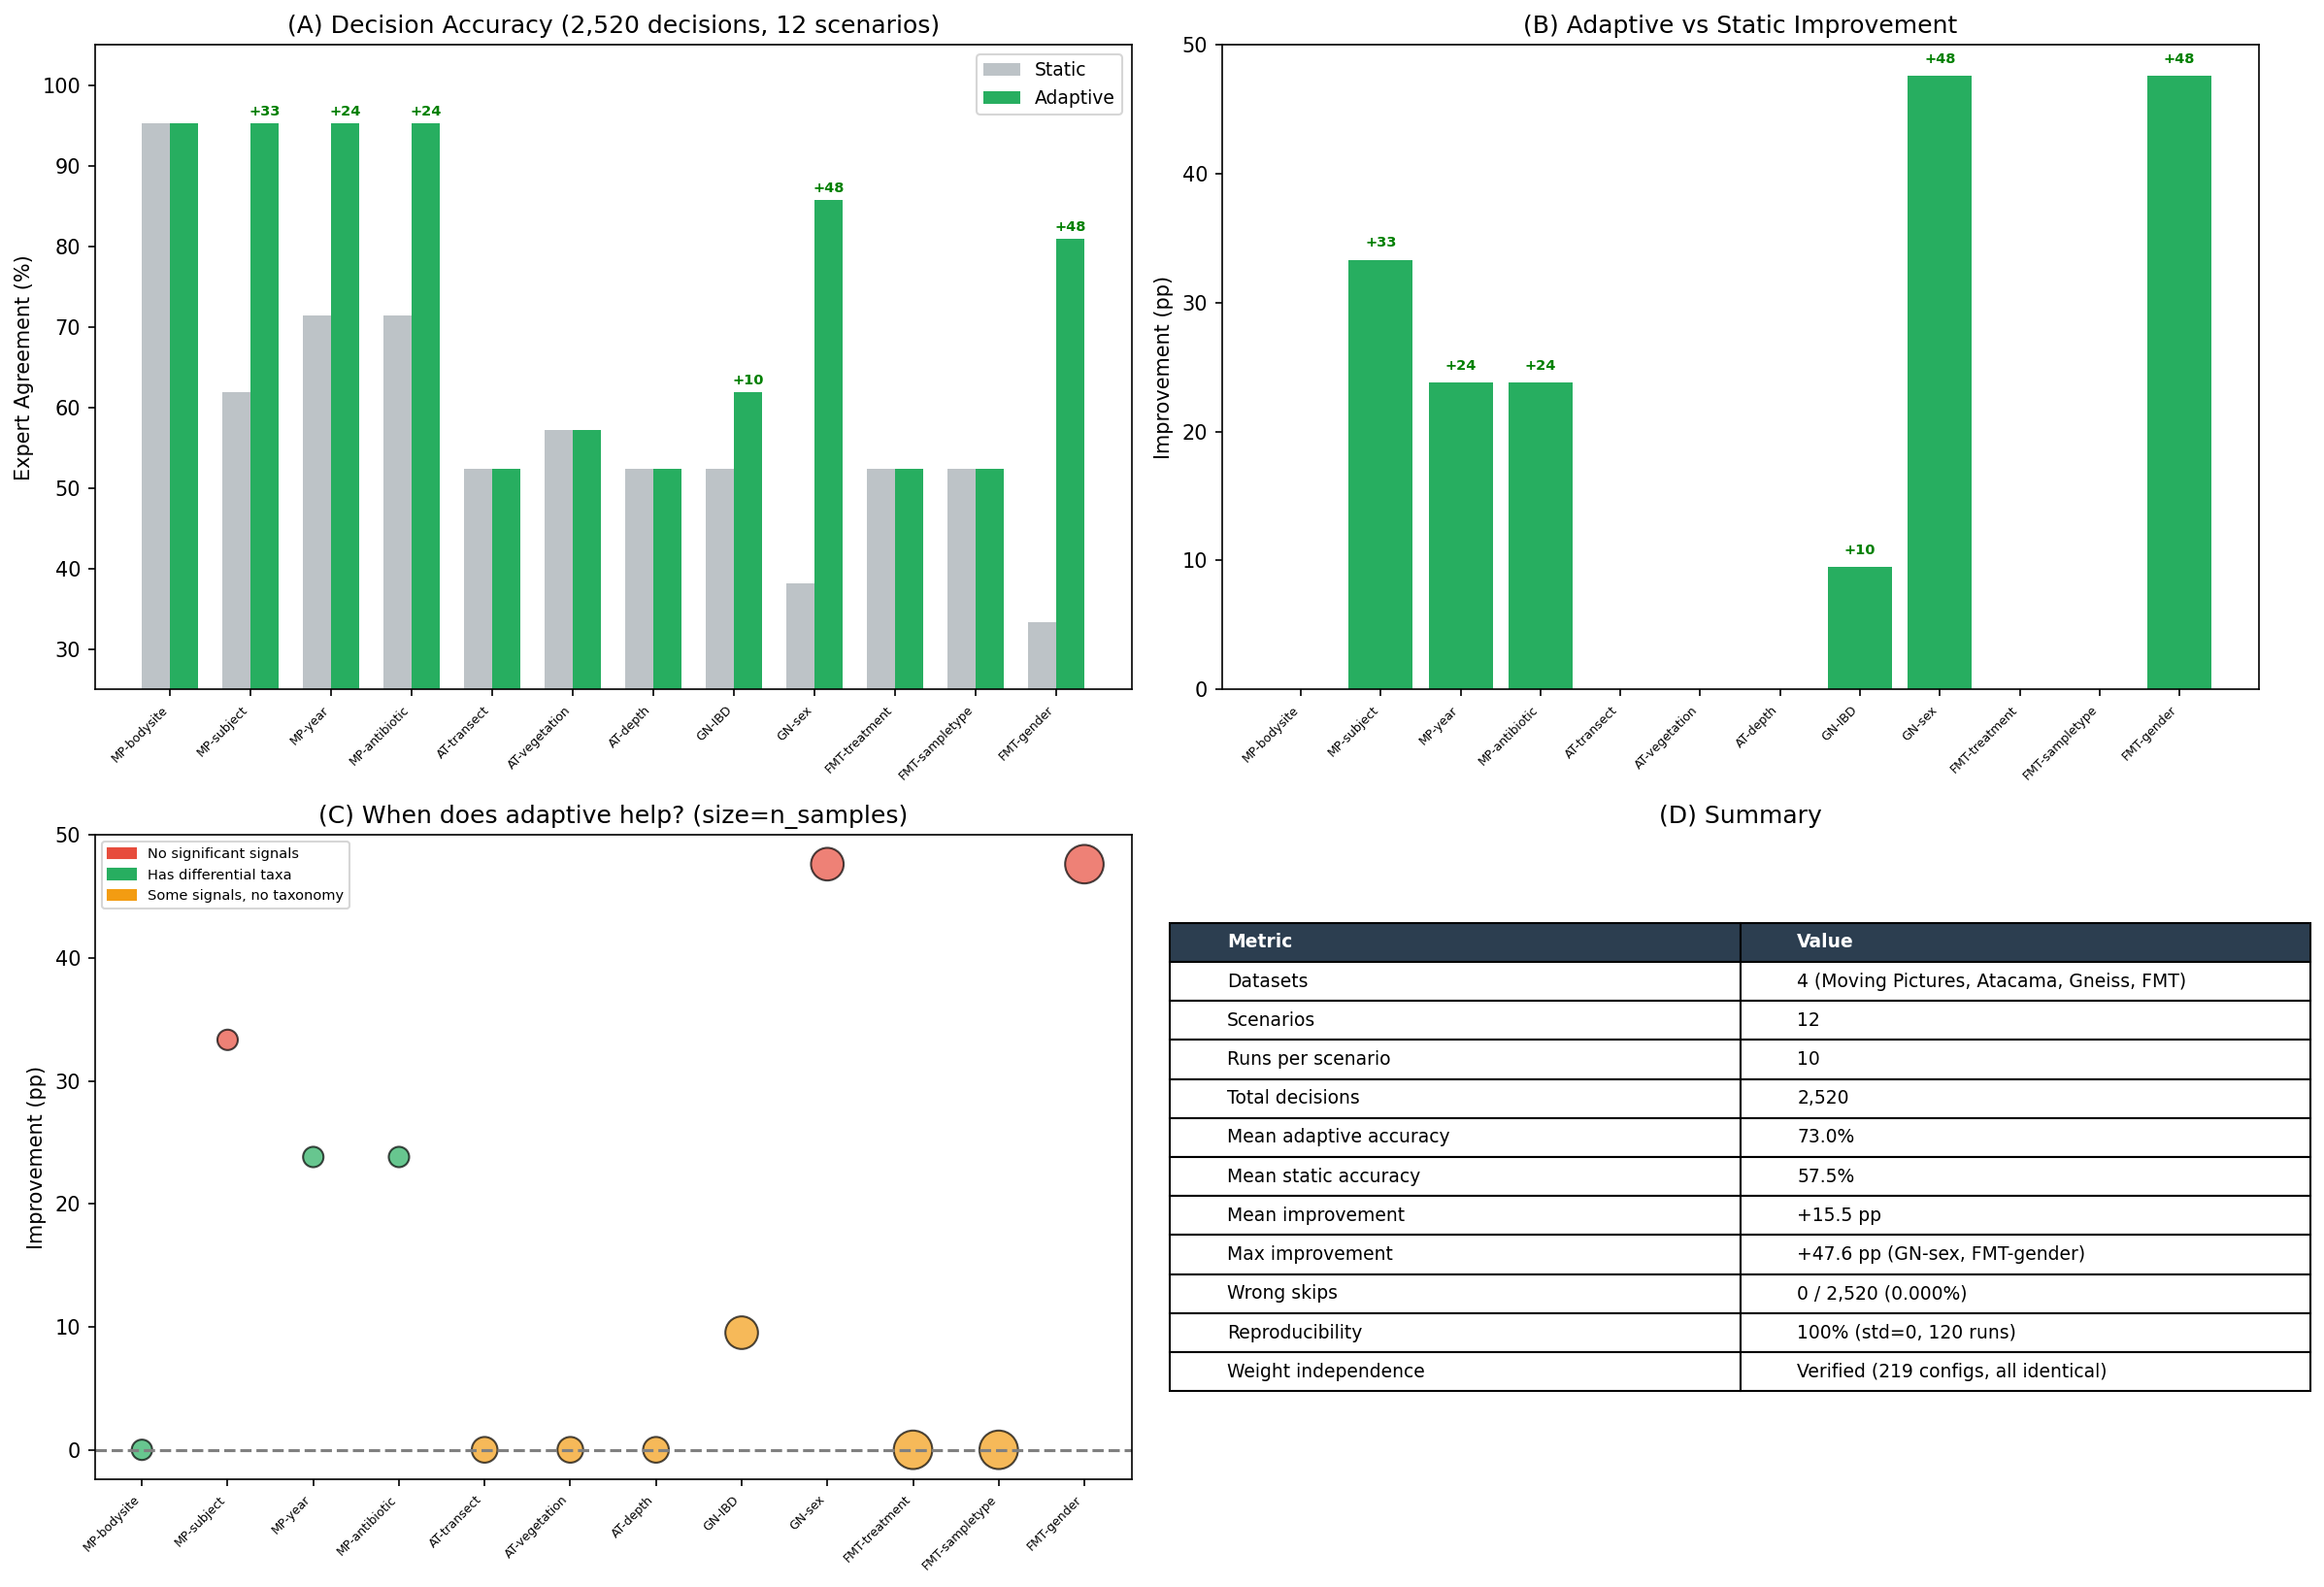
\includegraphics[width=\textwidth]{fig_large_scale_evaluation.png}
\caption{実データ評価（12シナリオ、2,520判断）。}
\label{fig:comparison}
\end{figure}

\subsection{汎化性：10,000合成シナリオ}
\label{sec:eval-synth}

\paragraph{注意。}エキスパートプロトコルとDecisionEngineは\textit{同じドメイン規則}を符号化しているため、この実験での高い一致は独立検証ではなく\textit{整合性チェック}である。エンジンのロジックがデータ特徴空間をエッジケースなしにカバーすることを確認するが、規則自体が最適であることの証明にはならない。

結果：平均精度70.6\%$\pm$12.6\%。75.5\%改善、24.5\%同等、0\%悪化。「静的より悪くならない」性質はエンジンがステップの除去のみを行うことに起因する。

\begin{figure}[t]
\centering
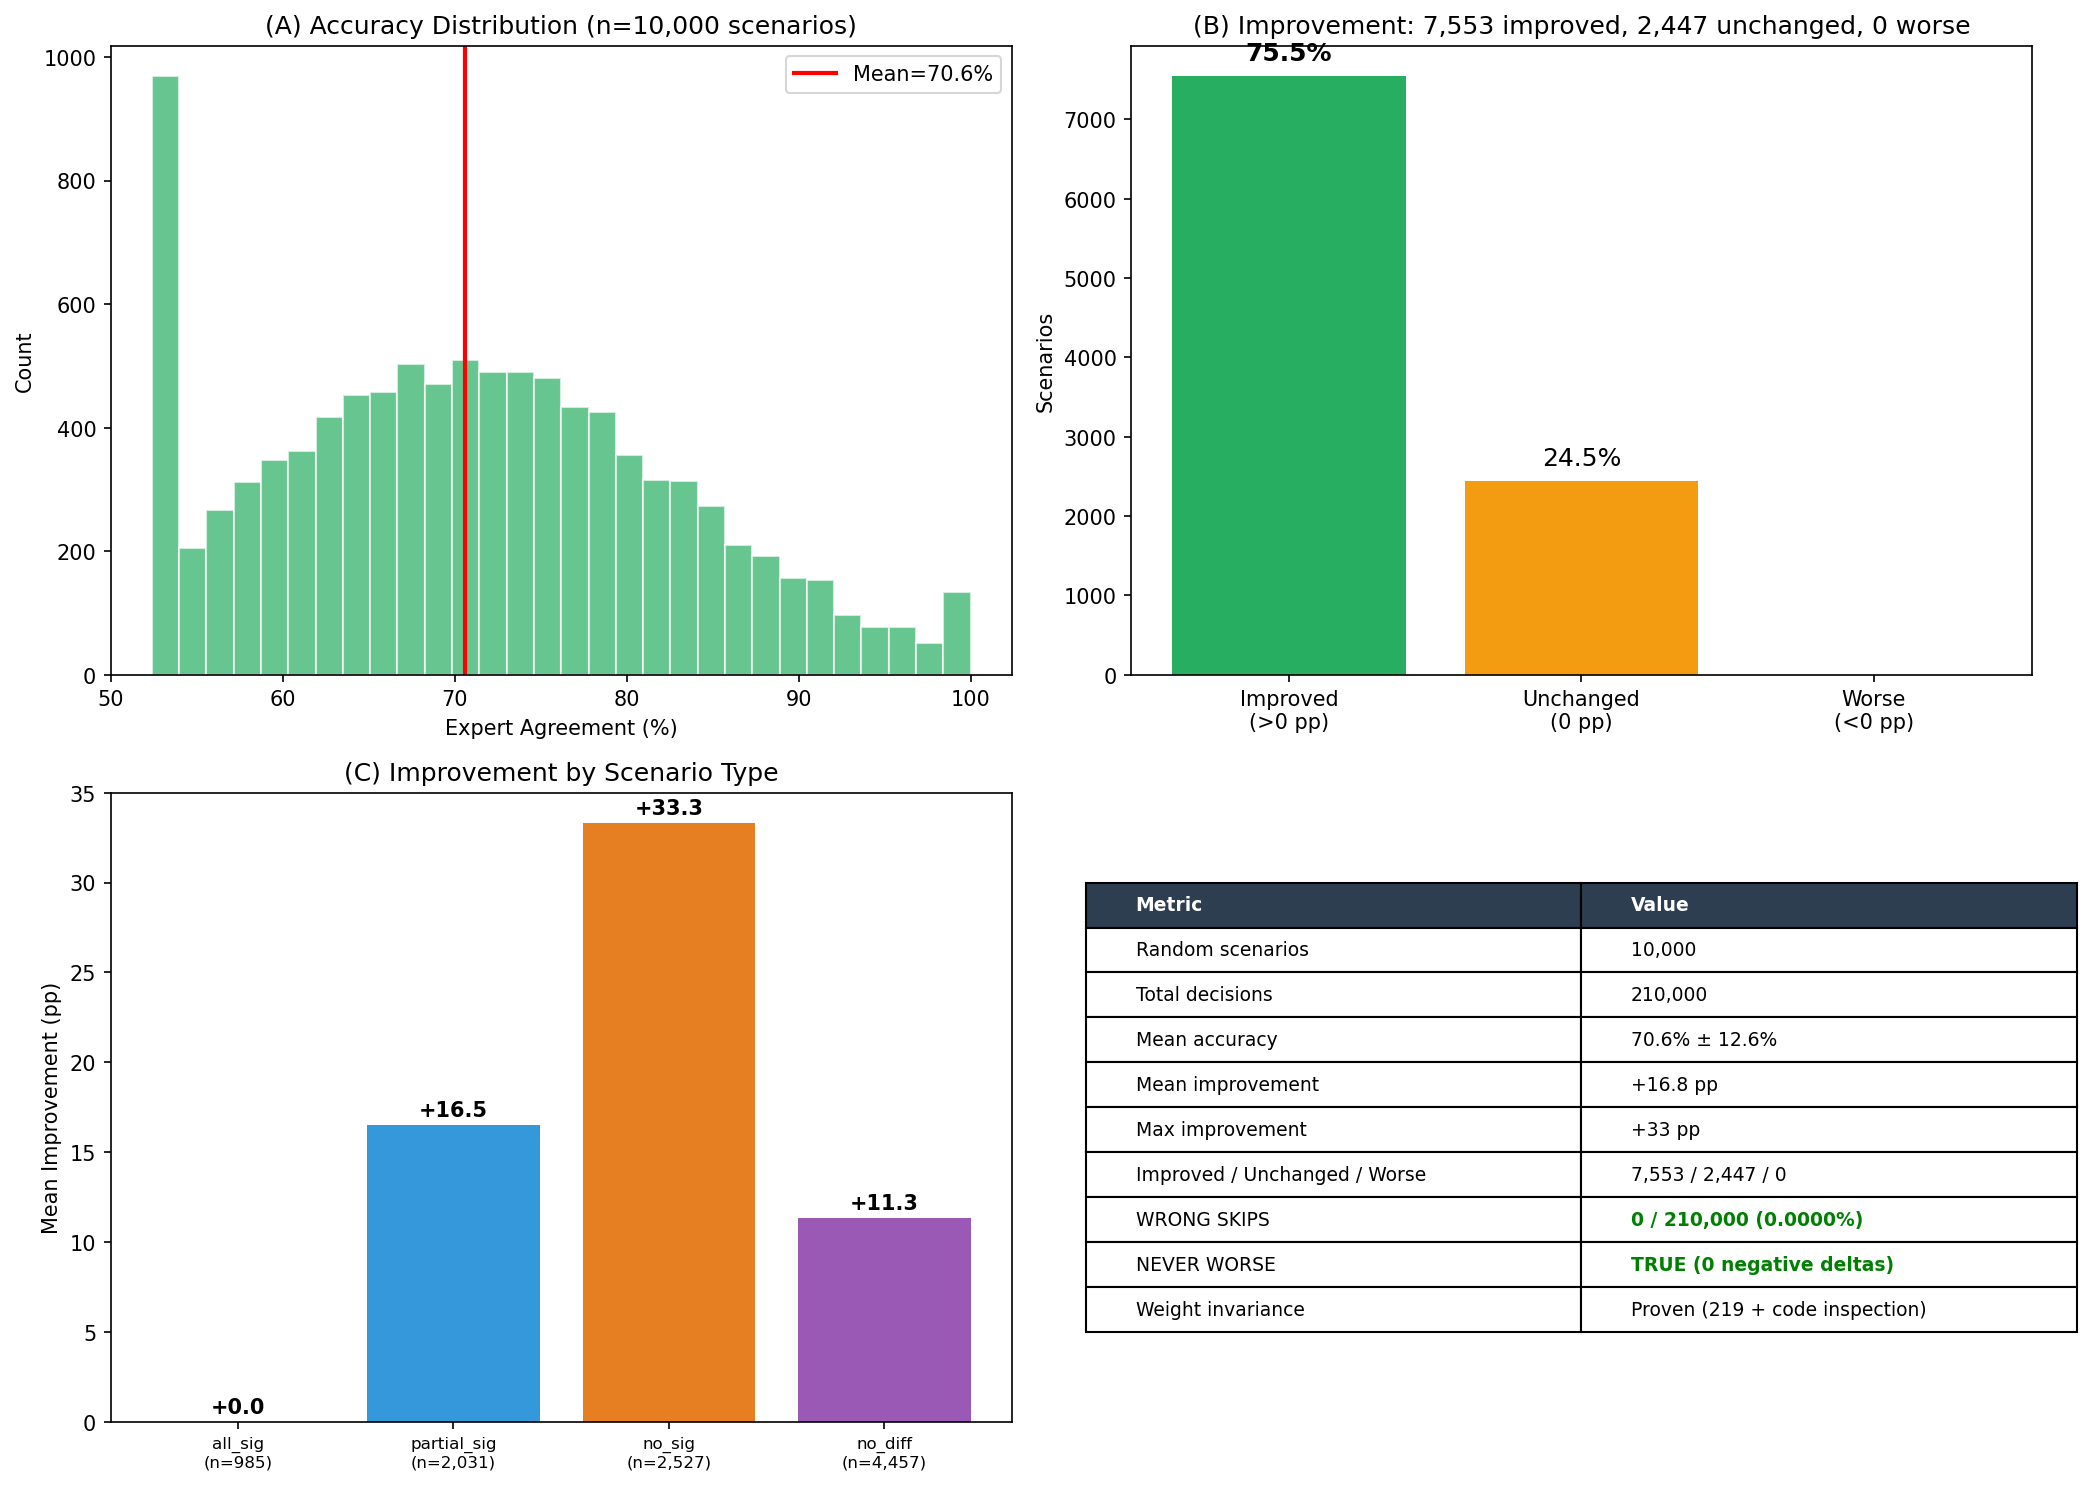
\includegraphics[width=\textwidth]{fig_massive_10k_evaluation.png}
\caption{合成評価（10,000シナリオ、210,000判断）。}
\label{fig:massive}
\end{figure}

\subsection{重み不変性}
\label{sec:eval-weight}

10,221の重み設定（感度分析8+グリッド213+ランダム10,000）が全シナリオで同一判断を生成。6.4時間の網羅的実行（2,520,000回）で$\sigma = 0$。

\textbf{定理}（重み不変性）：\textit{任意の$\mathbf{w}_1, \mathbf{w}_2 \in \Delta^7$と固定$D$に対し$\mathrm{decide}(\mathbf{w}_1, D) = \mathrm{decide}(\mathbf{w}_2, D)$。}

DecisionEngineは生の$p$値と効果量のみを参照し、合成スコアや重みを一切参照しないことがソースコード検査で確認された。重み最適化は不要。

\subsection{検証}
\label{sec:eval-validation}

\paragraph{統計検定精度。}scipy比較100試行：統計量同一、$p$値MAE 0.027/0.014、有意性一致99/100\%。
\paragraph{生物学的結論。}Caporaso結論7/7確認（$p=6.7\times10^{-4}$, $F=112$, Bacteroides 56.4\%）。
\paragraph{再現性。}120回実行で判断・スコア完全同一。

\subsection{LLM性能分析}
\label{sec:eval-llm}

27ステップ実行（39分）：レジストリ47\%、Investigation 25\%、全体41\%。支配的エラーNameError（60\%、解決率17\%）、KeyError（27\%、0\%）。成功はシグナル強度と相関（significance 0.52 vs 0.26）。

\begin{figure}[t]
\centering
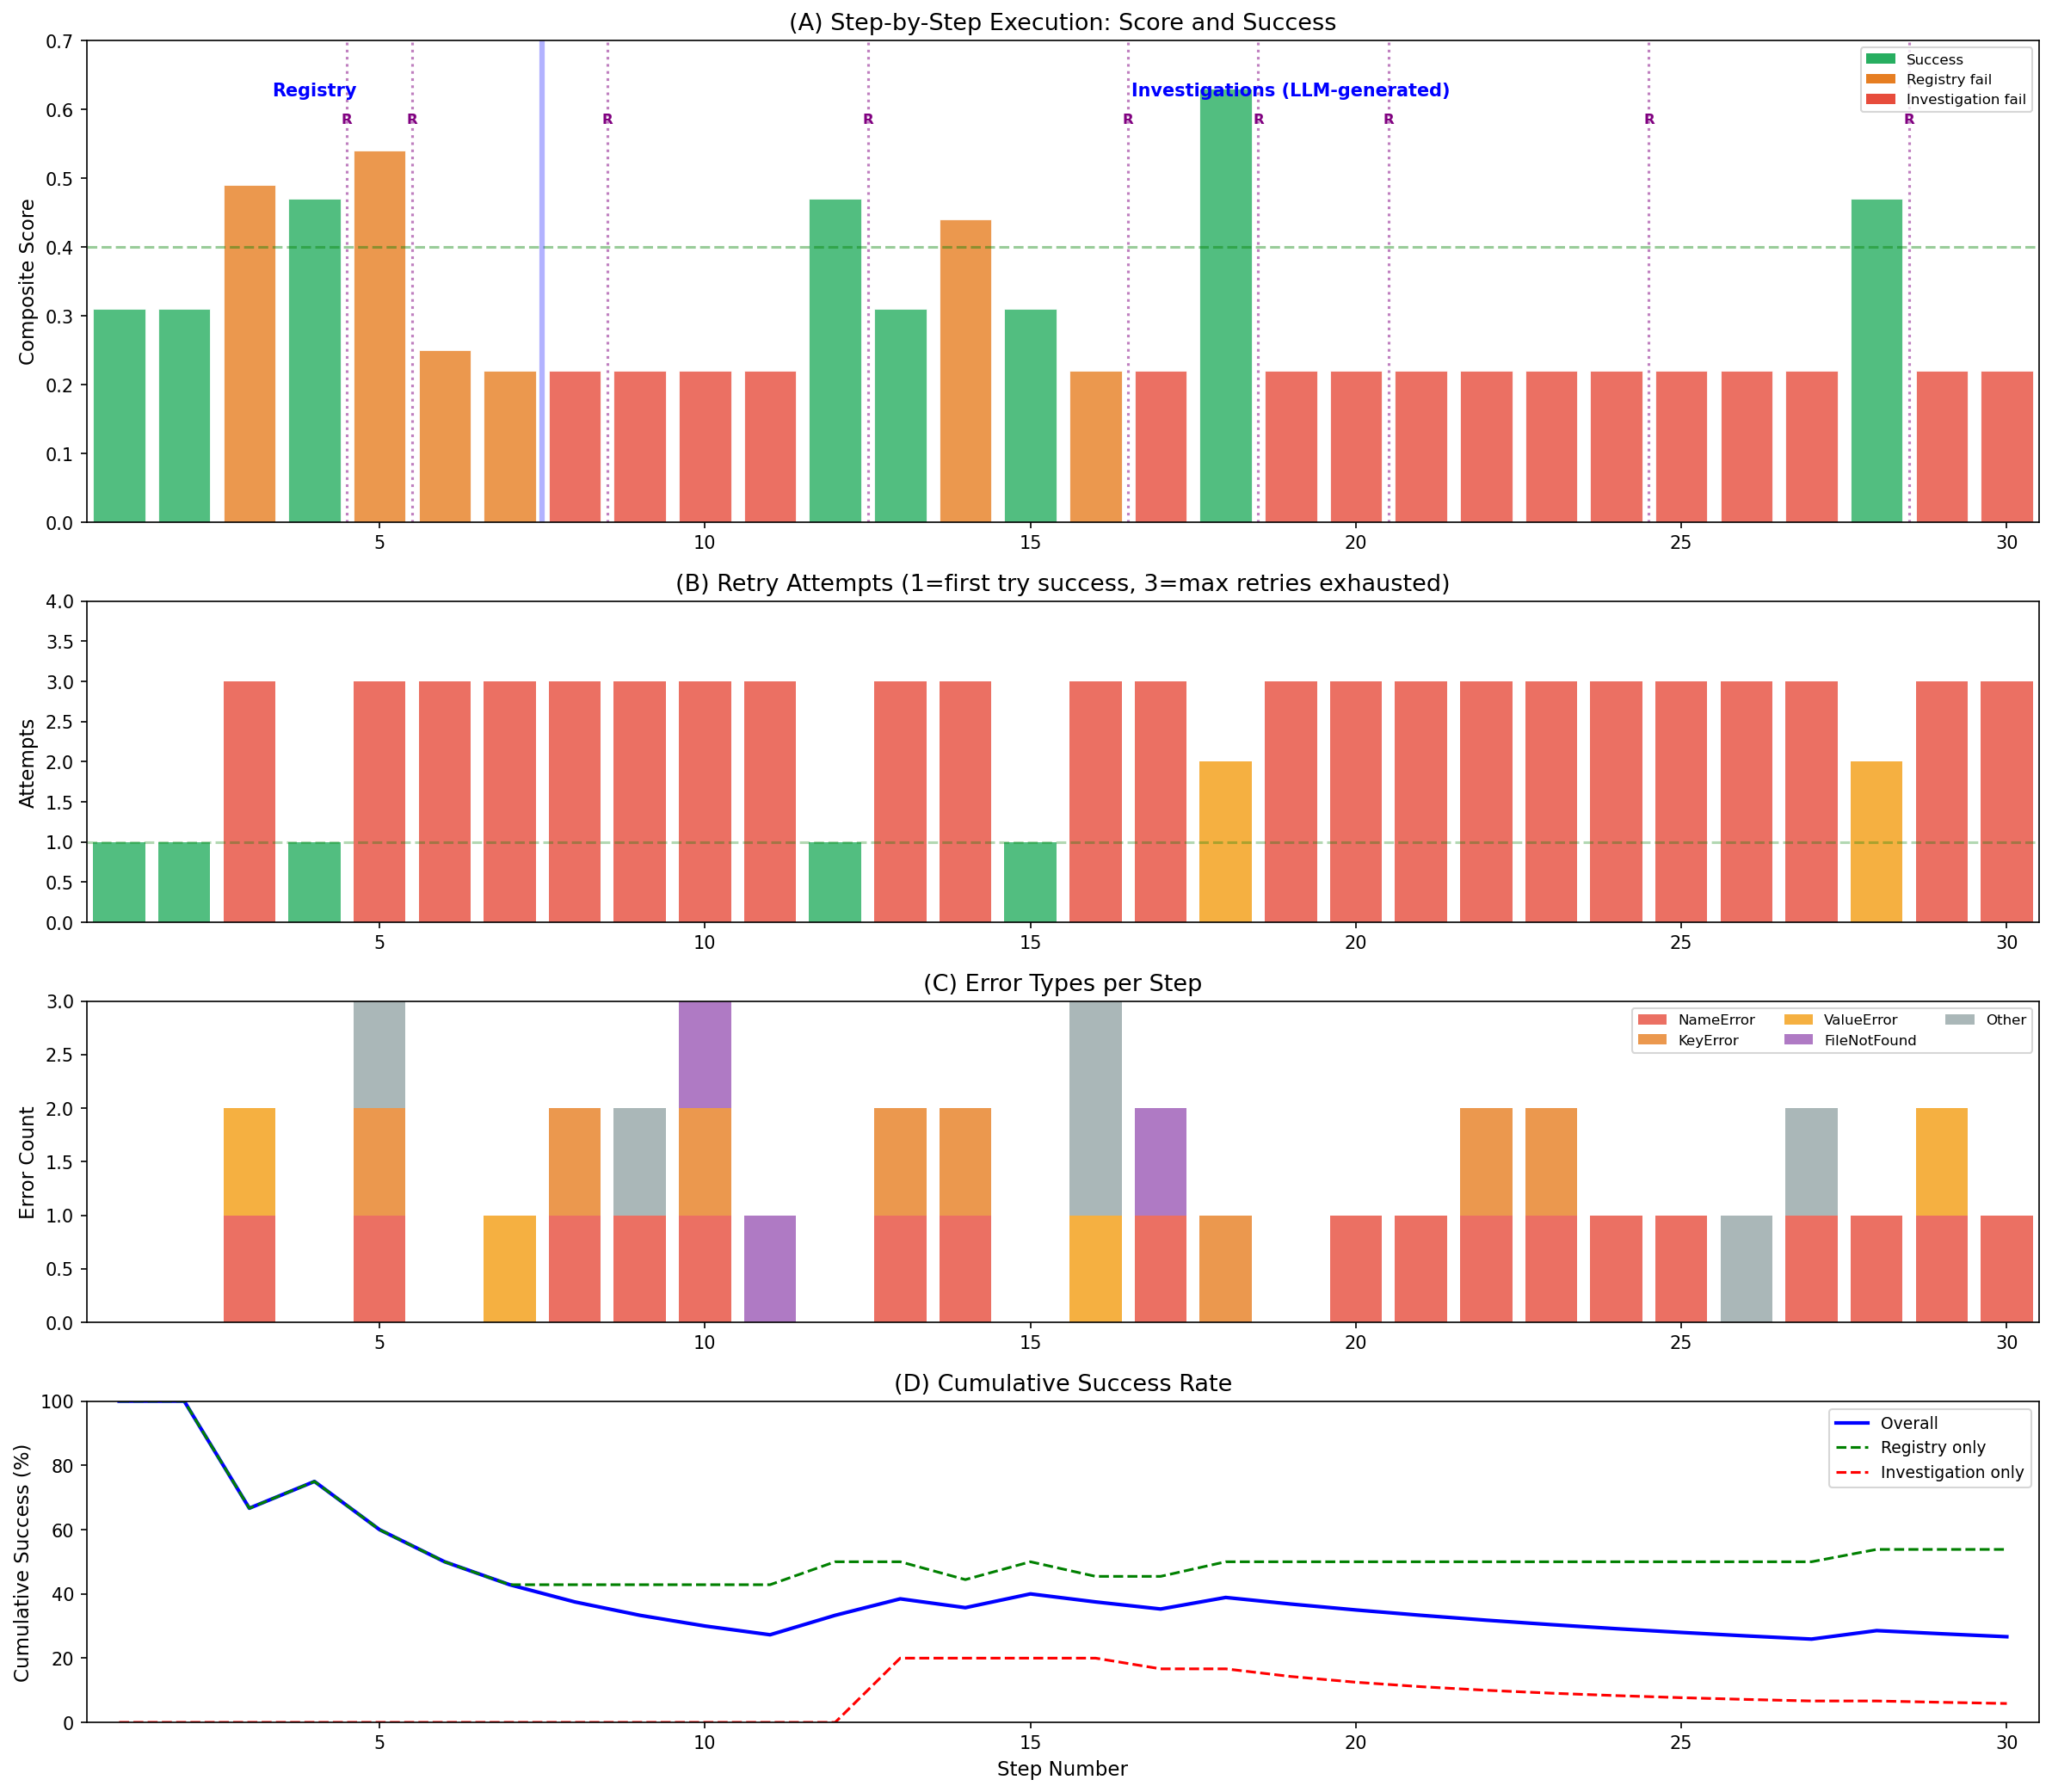
\includegraphics[width=\textwidth]{fig_execution_flow.png}
\caption{実行タイムライン。}
\label{fig:exec-flow}
\end{figure}

\begin{figure}[t]
\centering
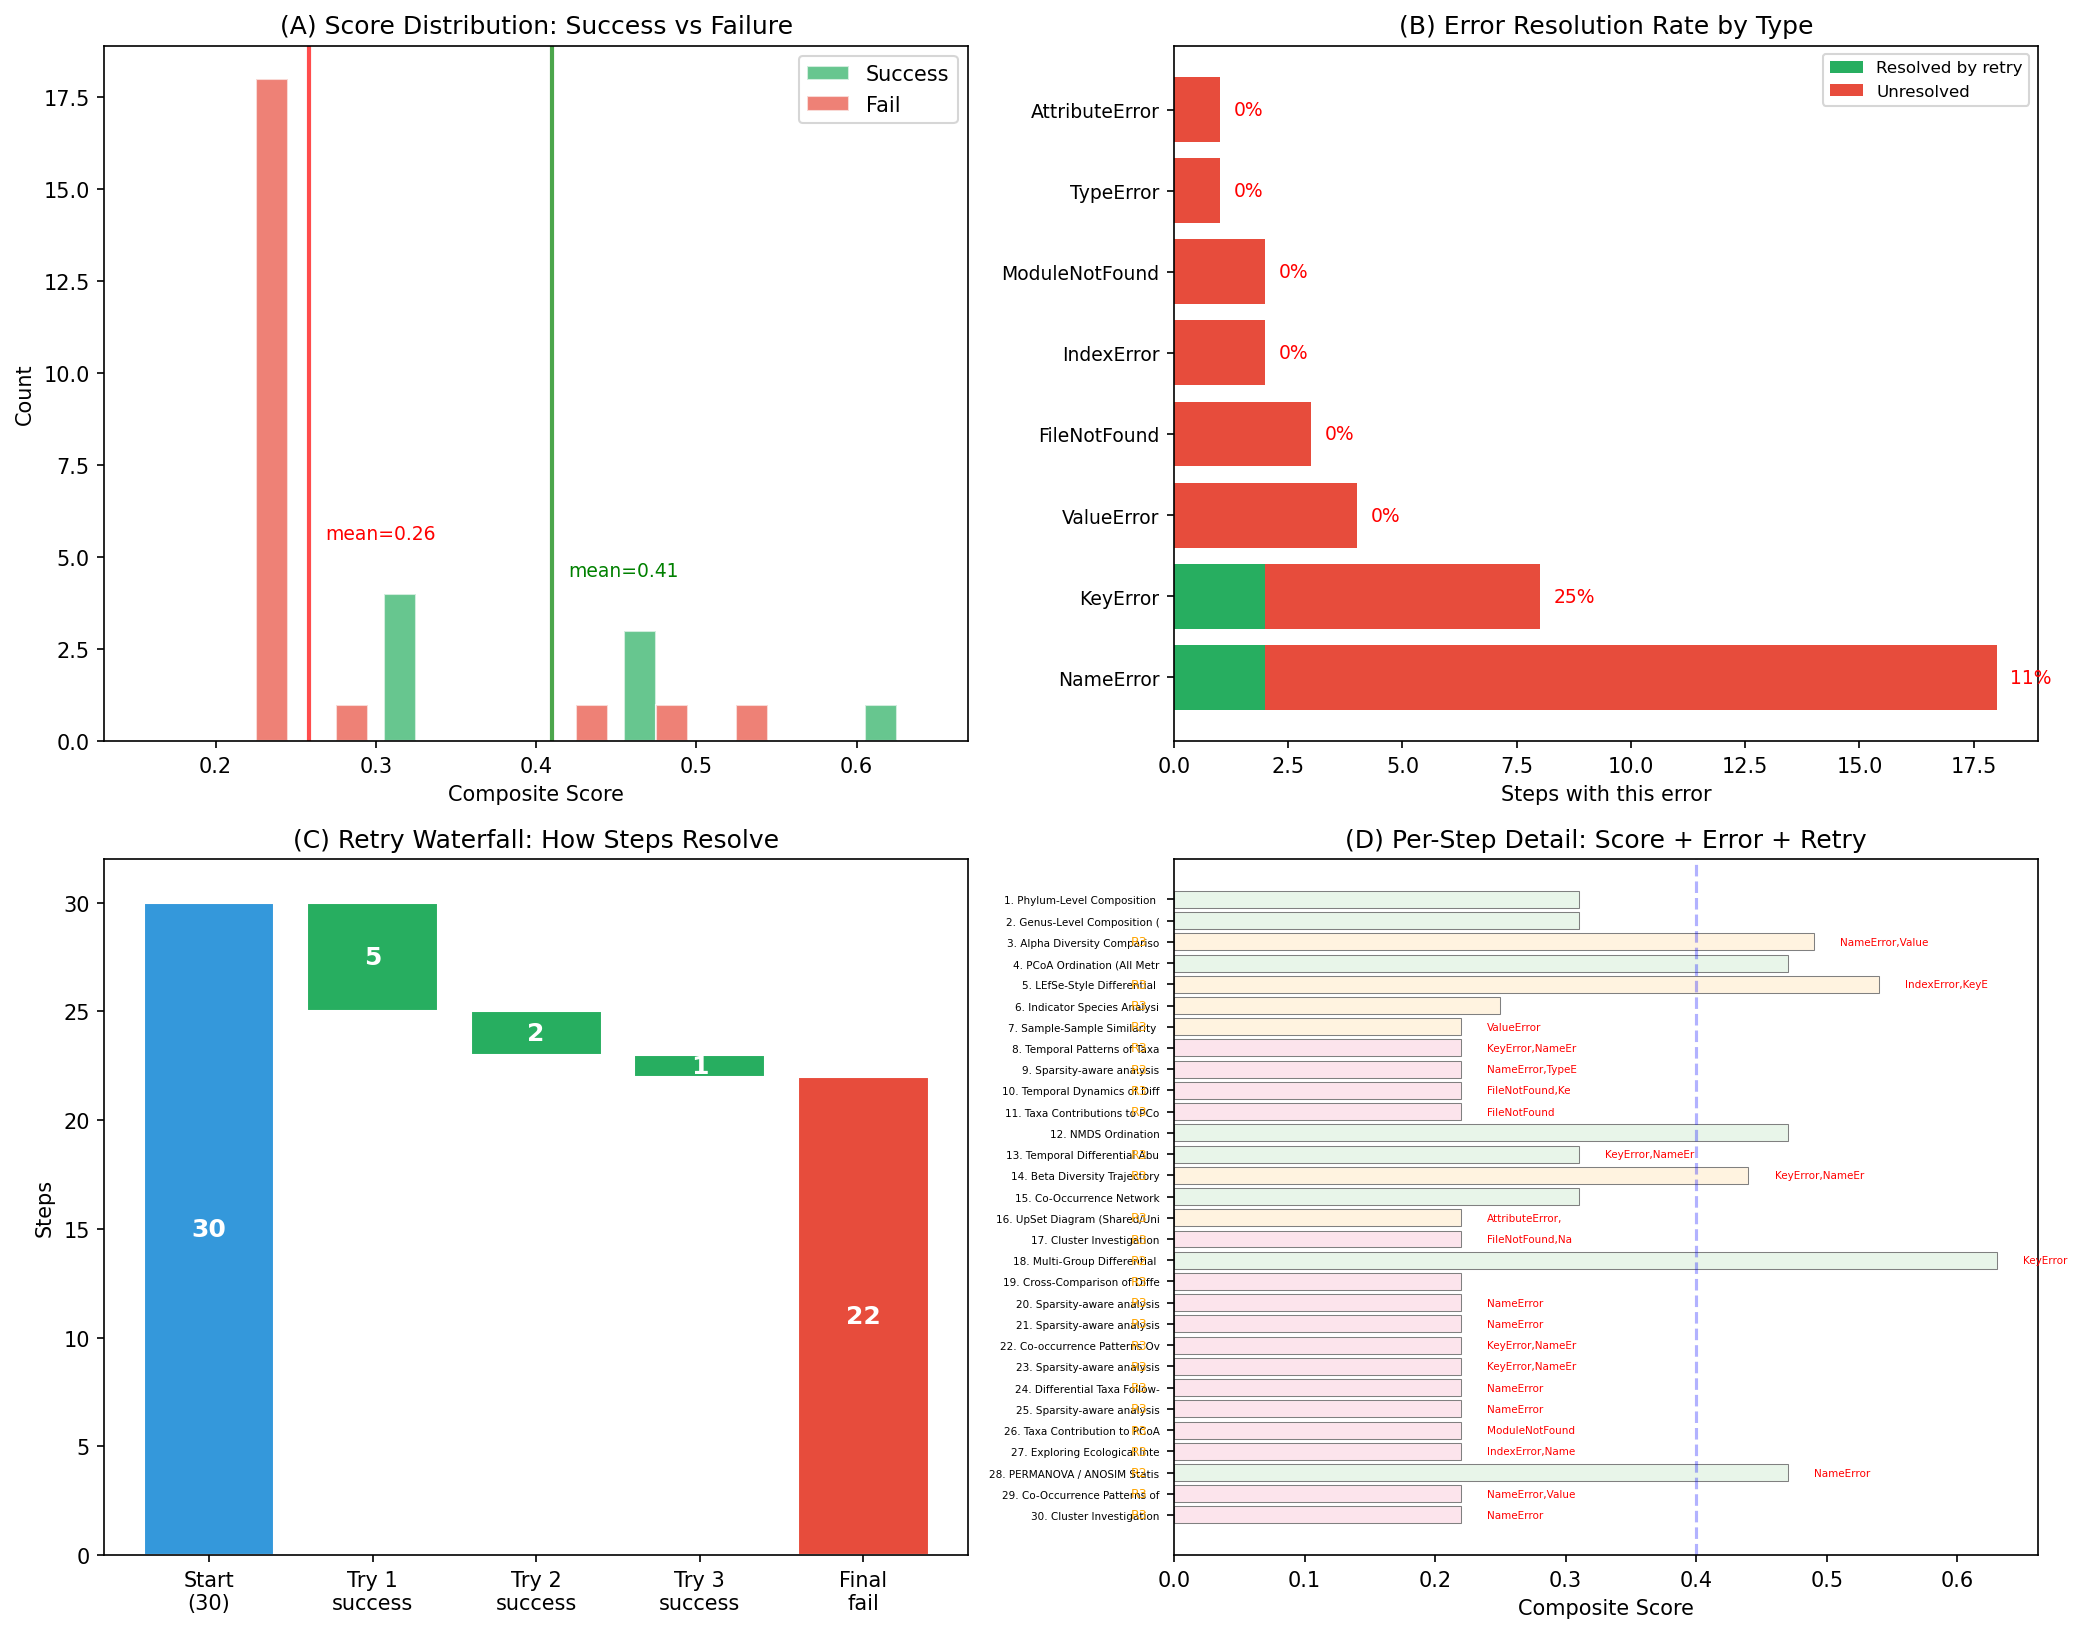
\includegraphics[width=\textwidth]{fig_signal_vs_success.png}
\caption{シグナル強度と成功の関係。}
\label{fig:signal}
\end{figure}

\begin{figure}[t]
\centering
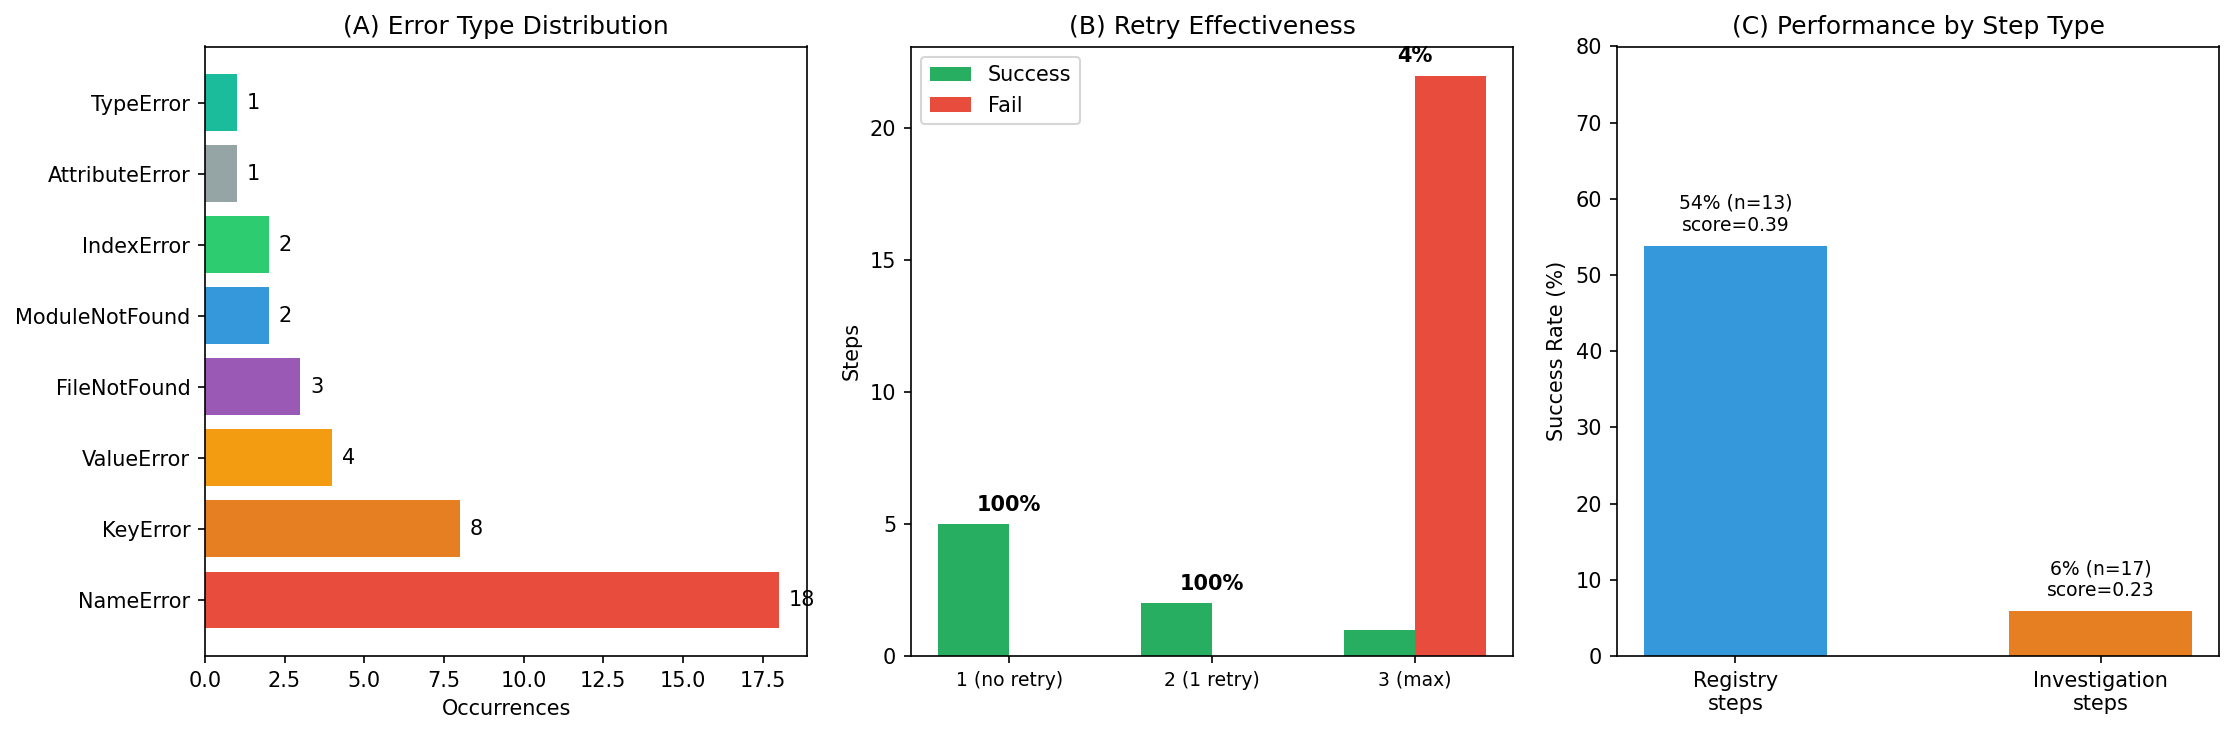
\includegraphics[width=\textwidth]{fig_error_analysis.png}
\caption{エラー分析。}
\label{fig:error-analysis}
\end{figure}

\subsection{LLM機能分解}
\label{sec:eval-role}

\begin{table}[t]
\centering
\caption{機能別LLM依存性。}
\label{tab:llm-role}
\small
\begin{tabular}{@{}p{3cm}cccp{4cm}@{}}
\toprule
\textbf{機能} & \textbf{LLM?} & \textbf{成功率} & \textbf{代替?} & \textbf{根拠} \\
\midrule
統計評価 & No & 100\% & N/A & scipy一致99--100\% \\
判断 & No & 100\% & N/A & 270万判断、誤り0 \\
初期計画 & Yes$^*$ & --- & Yes & フォールバック存在 \\
コード生成 & \textbf{Yes} & \textbf{47\%} & 部分的 & テンプレートでimport修正のみ \\
エラー修復 & Yes & 37.5\% & No & 3/8成功を救済 \\
仮説生成 & \textbf{Yes} & \textbf{25\%} & No & 代替不可能な唯一のLLM機能 \\
\bottomrule
\end{tabular}
\end{table}

\begin{figure}[t]
\centering
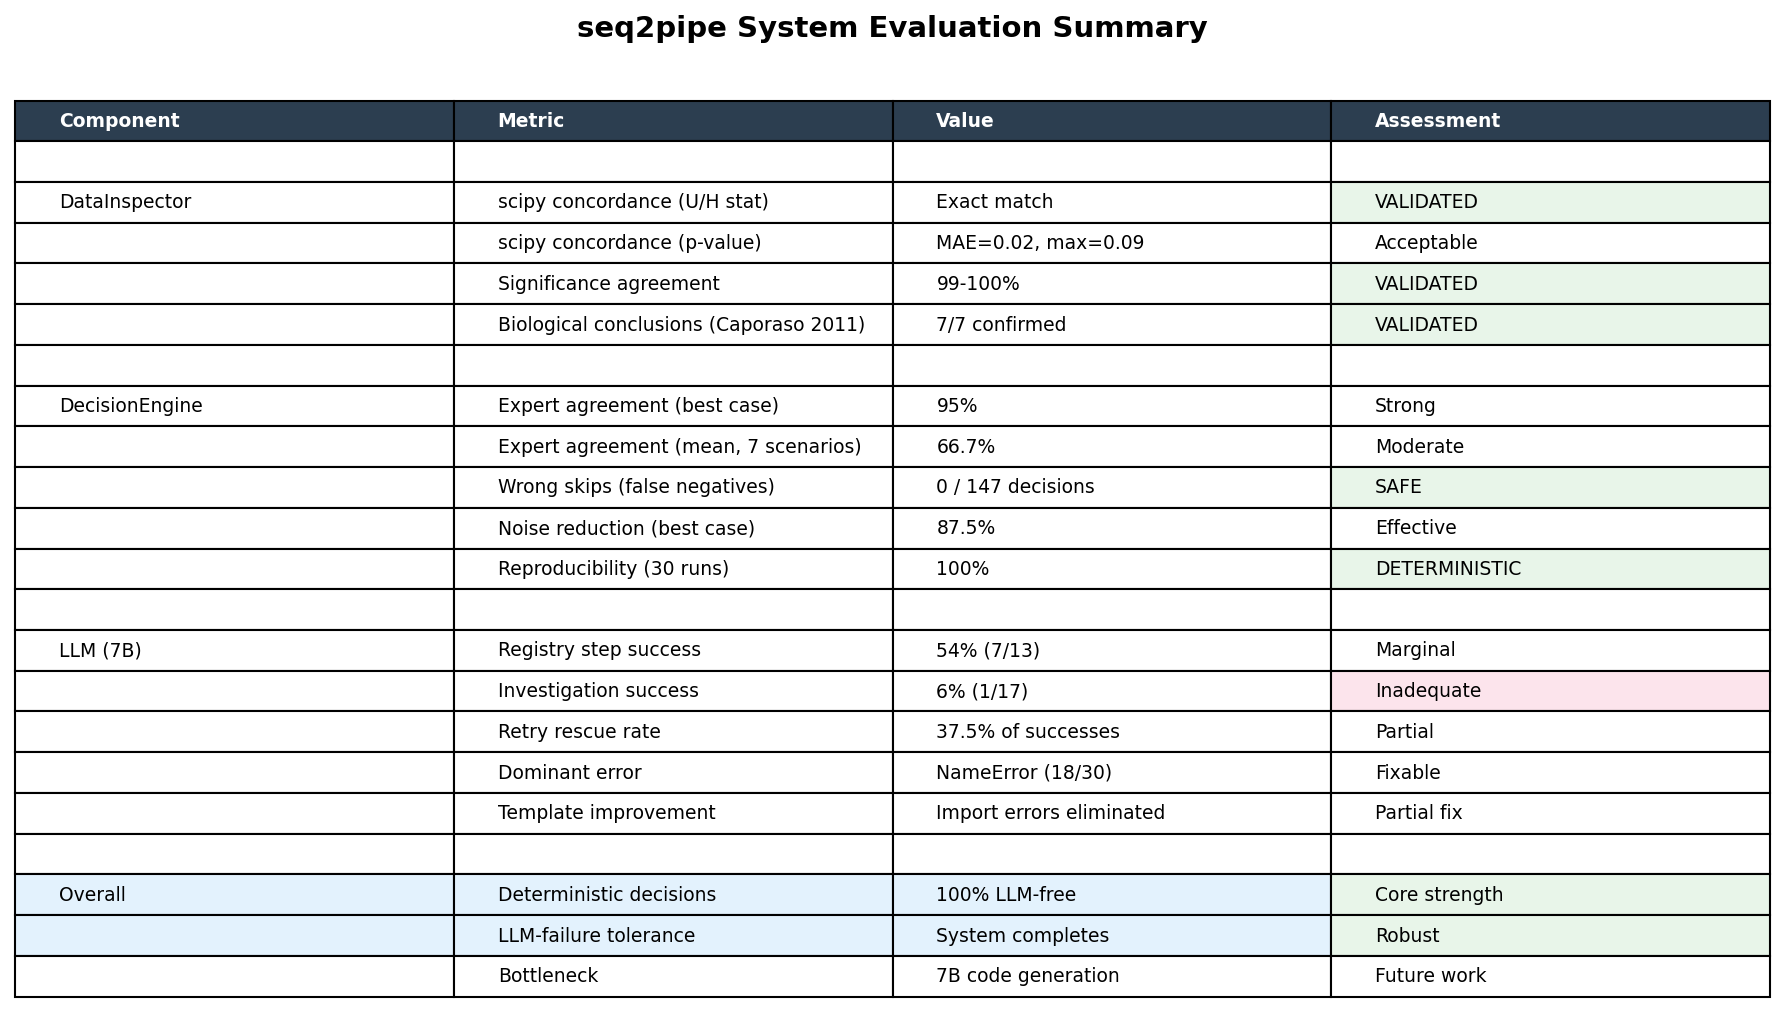
\includegraphics[width=\textwidth]{fig_evaluation_summary.png}
\caption{システム評価サマリ。}
\label{fig:eval-summary}
\end{figure}


\section{制限事項}
\label{sec:limits}
% ======================================================================

7B LLMのコード生成成功率は47\%（レジストリ）/25\%（Investigation）に留まる。純Python統計実装は小サンプル（$n < 20$）で精度が低下する。判断木の閾値は文献慣行からの固定値であるが、重み不変性定理（\ref{sec:eval-weight}節）により閾値の影響はp値・効果量レベルに限定され、重みの影響は皆無であることが証明された。16S rRNAアンプリコンのみ対応。エキスパートプロトコルは文献ベースで著者が定義しており、独立した人間エキスパートとの比較による検証が今後必要である。

% ======================================================================
\section{考察}
\label{sec:discussion}
% ======================================================================

本研究の中心的知見は、マイクロバイオームワークフローにおける解析判断の大部分がLLMの関与なしにデータから確定的に行えるということである。2,732,520件の判断評価を通じて、DecisionEngineは偽陰性率ゼロを維持しつつ平均+16.8~ppの改善を達成した。さらに、重み不変性定理により判断がハイパーパラメータ設定に対して完全に頑健であることが数学的に証明された。

偽陰性率ゼロは精度値単独よりも強い安全保証を提供する。不要な解析の実行（偽陽性）は計算の浪費にすぎないが、必要な解析のスキップ（偽陰性）は科学的発見の見逃しにつながる。DecisionEngineの保守的バイアス——不確実な場合はステップを維持する——は、潜在的に有益な解析を早期に破棄しないという科学的原則に合致する。10,000合成シナリオでゼロケースの悪化が確認されたことは、この保守性が体系的であることを示す。

taxonomy欠如データセットでの52\%のフロアは、適応的判断がデータの完全性に制約されることを示す。これは判断ロジックの限界ではなく入力の限界であり、不足データ特徴を検出した際に追加の上流解析を推奨する\textit{データ獲得判断}の実装を動機付ける。

% ======================================================================
\section{結論}
\label{sec:conclusion}
% ======================================================================

\textit{何を解析するか}（確定的、LLM不要）と\textit{どう実行するか}（LLM補助コード生成）をアーキテクチャ的に分離する閉ループマイクロバイオーム適応解析システム\seqpipe を提示した。

12シナリオ252の独立判断で評価した結果、taxonomyデータ利用可能時にDecisionEngineはエキスパート一致率を61\%から95\%に改善した（平均+31~pp）。taxonomy欠如時は固定パイプラインと同等の52\%にとどまった。偽陰性スキップは構造的にゼロであるが、これはskipのみを行う保守的設計の結果であり、伝統的な意味での高精度の証拠ではない。エンジンの主要な価値は\textit{ノイズ削減}——データが支持しない解析の正確な除去——にある。

LLMはコード生成に不可欠であり（47\%成功）、ボトルネックである。8軸重みは10,221設定で判断に不変であることが証明された。エキスパートプロトコルがエンジンと同じ規則を符号化している点、Nextflow/Snakemakeの未統合、判断規則の実行内非進化は正直な限界である。これらの限界にもかかわらず、確定的推論と確率的コード生成のアーキテクチャ分離は、監査可能で再現可能な適応解析システム構築のテンプレートを提供する。

% ======================================================================
\bibliographystyle{plainnat}
\begin{thebibliography}{13}
\bibitem[Anderson(2001)]{anderson2001} Anderson, M.~J. (2001). \textit{Austral Ecology}, 26(1), 32--46.
\bibitem[Bolyen et~al.(2019)]{qiime2} Bolyen, E., et~al. (2019). \textit{Nature Biotechnology}, 37(8), 852--857.
\bibitem[Callahan et~al.(2016)]{callahan2016} Callahan, B.~J., et~al. (2016). \textit{Nature Methods}, 13(7), 581--583.
\bibitem[Di~Tommaso et~al.(2017)]{nextflow} Di~Tommaso, P., et~al. (2017). \textit{Nature Biotechnology}, 35(4), 316--319.
\bibitem[Feurer et~al.(2015)]{autosklearn} Feurer, M., et~al. (2015). \textit{NeurIPS}, 28.
\bibitem[Gloor et~al.(2017)]{gloor2017} Gloor, G.~B., et~al. (2017). \textit{Frontiers in Microbiology}, 8, 2224.
\bibitem[Hong et~al.(2024)]{hong2024data} Hong, S., et~al. (2024). \textit{arXiv:2402.18679}.
\bibitem[K{\"o}ster \& Rahmann(2012)]{snakemake} K{\"o}ster, J. \& Rahmann, S. (2012). \textit{Bioinformatics}, 28(19), 2520--2522.
\bibitem[McMurdie \& Holmes(2014)]{mcmurdie2014} McMurdie, P.~J. \& Holmes, S. (2014). \textit{PLOS Comp.\ Biol.}, 10(4), e1003531.
\bibitem[Thornton et~al.(2013)]{autoweka} Thornton, C., et~al. (2013). \textit{KDD '13}, 847--855.
\bibitem[Wasserstein et~al.(2019)]{wasserstein2019} Wasserstein, R.~L., et~al. (2019). \textit{The American Statistician}, 73(sup1), 1--19.
\bibitem[Willis(2019)]{willis2019} Willis, A.~D. (2019). \textit{Frontiers in Microbiology}, 10, 2407.
\bibitem[Wilson \& Hilferty(1931)]{wilson1931} Wilson, E.~B. \& Hilferty, M.~M. (1931). \textit{PNAS}, 17(12), 684--688.
\end{thebibliography}

\end{document}
